\section{ZÁKLADNÍ VZTAHY PRO VÝPOČET CHYB V ANALOGOVÝCH OBVODECH }
Princip superpozice, celková chyba součtu a součinu dvou chybových veličin, přepočet chyb v obvodu diferenčního zapojení (výpočet vstupní napěťové nesymetrie komparátoru s BJT při známé chybě saturačního proudu vstupních tranzistorů)

\subsection{Princip superpozice}
Máme systém, který je charakterizován nějakou veličinou Q (např. offset, výstupní napětí,..). Chyba veličiny Q je dána několika dílčími nekorelovanými chybami uvnitř tohoto systému. Celková chyba veličiny Q se počítá tak, že se postupně vyjádří vliv každé dílčí chyby na veličinu Q, při tom se ostatní dílčí chyby zanedbají - položí rovno 0. Nakonec se vlivy všech dílcích chyb nekorelovaně sečtou a tím se získá celková chyba (rozptyl) veličiny Q.

\subsection{Příklad součtu výstupních proudů z proudových zrcadel}

\begin{figure}[h]
   \begin{center}
     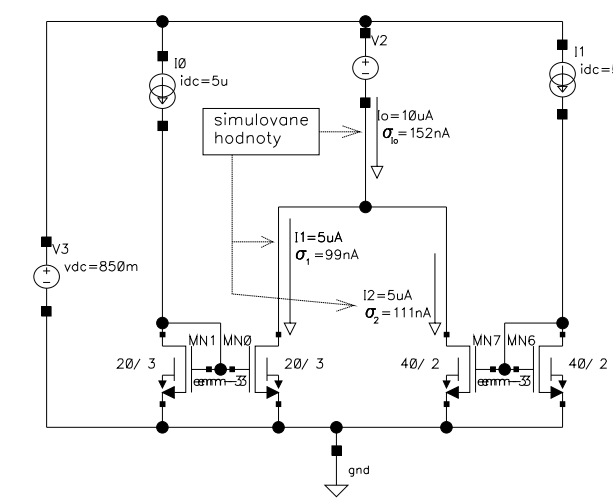
\includegraphics[scale=0.5]{images/Chyba_Souctu.png}
   \end{center}
   \caption{Chyba součtu dvou veličin}
\end{figure}

Mějme dvě veličiny I\textsubscript{1} a I\textsubscript{2}, které jsou vzájemně nekorelované (nijak na sobě nezávisí). Proud I\textsubscript{1} nikterak nezávisí na proudu I\textsubscript{2} a naopak. Velikost těchto proudů je zatížena chybou ($\sigma$\textsubscript{1} a $\sigma$\textsubscript{2}).

Chyba $\sigma$ součtu proudů se potom vypočítá jako:
\begin{equation}
\sigma = \sqrt{\sigma_{1}^{2}+\sigma_{2}^{2}}
\end{equation}

Při sčítání nekorelovaných veličin je jedna důležitá vlastnost. Pokud je jedna veličina menší než 1/2 největší veličiny, ve výsledku se téměř neprojeví (dá se zanedbat), protože zvýší výslednou hodnotu jen asi o desetinu.

Mějme: x\textsubscript{1} = 1 a x\textsubscript{2} = 0,5. Potom:
\begin{equation}
\sigma = \sqrt{\sigma_{1}^{2}+\sigma_{2}^{2}}=\sqrt{1^{2}+0,5^{2}}=1,12\doteq 1
\end{equation}

\subsection{Příklad součinu výstupních proudů z proudových zrcadel}
\begin{figure}[h]
   \begin{center}
     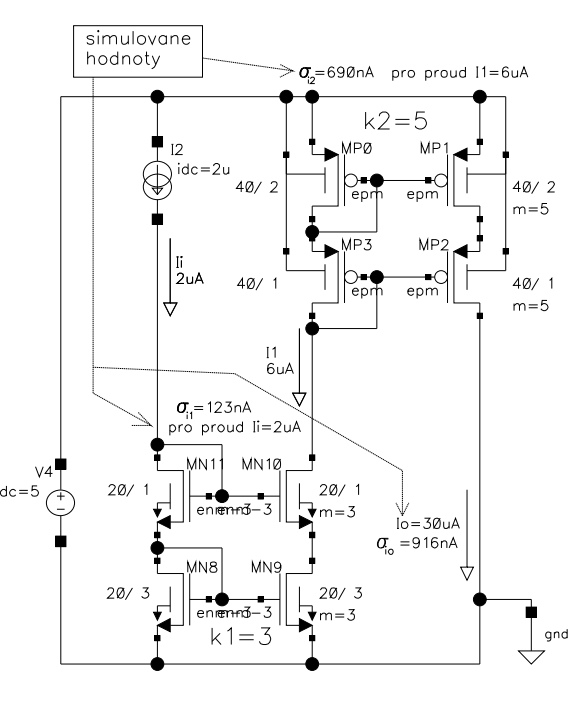
\includegraphics[scale=0.5]{images/Soucin.png}
   \end{center}
   \caption{Chyba součinu}
\end{figure}

První zrcadlo má přesnost K\textsubscript{1}=3 a chyba tohoto přenosu je I\textsubscript{i}= 2 $\mu$A vyjádřená jako odchylka výstupního proudu od očekávané hodnoty
\begin{equation}
I_{1}=k_{1}*I_{i}=6\mu A => \sigma_{i1}=123nA
\end{equation}

Pro skutečnou hodnotu K\textsubscript{1} přenosu k\textsubscript{1} pak můžeme napsat:
\begin{equation}
K_{1} = \frac{I_{1}+\sigma_{i1}}{I_{i}}=\frac{k_{1}*I_{i}+\sigma_{i1}}{I_{i}} = k_{1}+\frac{\sigma_{i1}}{I_{i}}
\end{equation}
, kde $\sigma$\textsubscript{1} = $\sigma$\textsubscript{i1}/I\textsubscript{i}.

Pro úvahu o chybě přenosu K\textsubscript{2}=5 nyní předpokládejme, že druhé zrcadlo měříme za stejných podmínek jako v daném zapojení, tedy jeho vstupní proud I\textsubscript{1}=6 $\mu$A. Pro skutečnou hodnotu K\textsubscript{2} přenosu k\textsubscript{2} pak můžeme napsat:
\begin{equation}
K_{2} = \frac{I_{o}+\sigma_{i2}}{I_{1}}=\frac{k_{2}*I_{1}+\sigma_{i2}}{I_{1}} = k_{2}+\frac{\sigma_{i2}}{I_{1}}
\end{equation}
, kde $\sigma$\textsubscript{2} = $\sigma$\textsubscript{i2}/I\textsubscript{1}.
K\textsubscript{2} je skutečná hodnota přenosu K\textsubscript{2}.

Celkovou chybu $\sigma$\textsubscript{io} vstupního proudu I\textsubscript{o} pak můžeme vyjádřit jako nekorelovaný součet těchto dvou chyb:
\begin{equation}
\sigma_{io}=k_{1}*k_{2}*I_{i}*\sqrt{(\frac{\sigma_{2}}{k_{2}})^2+({\frac{\sigma_{1}}{k_{1}}})^2}
\end{equation}



\subsection{Přepočet chyb v obvodu diferenčního zapojení}

\begin{figure}[h]
   \begin{center}
     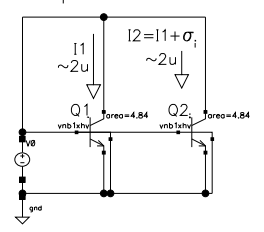
\includegraphics[scale=1]{images/Prepocet.png}
   \end{center}
   \caption{Chyba vstupního proudu}
\end{figure}

Měření probíhá na teoreticky identických tranzistorech Q1 a Q2. Měřením je zjištěn rozdíl proudů (odchylky), kdy z této odchylky můžeme spočítat chybu $\sigma$I\textsubscript{1}/I\textsubscript{2} poměru proudů I\textsubscript{1} a I\textsubscript{2}:
\begin{equation}
I_{2} = I_{1}+\sigma_{1} => \frac{I_{2}}{I_{1}} = \frac{I_{1}+\sigma_{i}}{I_{1}}=1+\frac{\sigma_{i}}{I_{1}} => \frac{\sigma_{i}}{I_{1}} = \sigma_{I1/I2}
\end{equation}

Z tohoto výpočtu potom můžeme na základě úvahy "o kolik musíme změnit U\textsubscript{be} tranzistoru Q1, aby proud I\textsubscript{1} byl stejný jako proud I\textsubscript{2}" určit nesouběh Ube dvou identických tranzistorů. Jinak řečeno, určíme rozdíl U\textsubscript{be} těchto dvou tranzistorů pro případ, kdy hodnota proudu I\textsubscript{2} je přesně rovna prudu I\textsubscript{1}:
\begin{equation}
\sigma_{dUbe} = U_{T}*ln(1+\sigma_{I1/I2})
\end{equation}

\begin{figure}[h]
   \begin{center}
     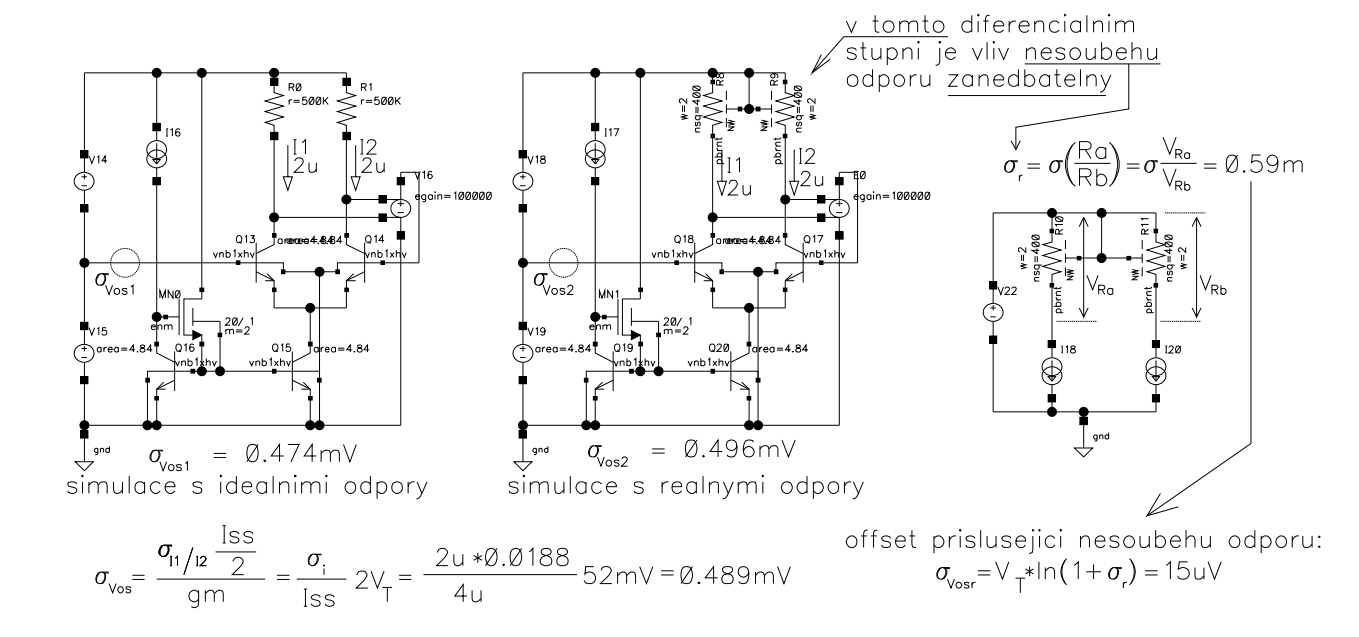
\includegraphics[scale=0.4]{images/Soubeh.png}
   \end{center}
   \caption{Reálná simulace nesymetrie}
\end{figure}

























